%% June 2016
%% ENOC2017 template file for LaTeX modified by Gabor Csernak, Budapest University of Technology and Economics and 
%% Horst Ecker, Vienna University of Technology
%% based on ENOC2011 template file for LaTeX generated by Andrea Arena, Sapienza University of Rome
%% This file was generated with a LateX2e version.
%%%%%%%%%%%%%%%%%%%%%%%%%%%%%%%%%%%%%%%%%%%%%%%%%%%%%%%%%%%%
\documentclass[10pt]{enoc2017}
\usepackage{epsfig,amsmath,amsfonts}
\usepackage{cite}
\usepackage{amsthm}
\usepackage{amssymb}
\usepackage[font=small]{caption}
\usepackage{tikz}
\usepackage{mdframed}
\usetikzlibrary{plotmarks}
\usepackage{hyperref}
\newtheorem{proposition}{Proposition}
\newtheorem{theorem}{Theorem}
\newtheorem{definition}{Definition}
\newtheorem{lemma}{Lemma}
\newtheorem{alg}{Algorithm}

\newenvironment{falg}
{\begin{mdframed}\begin{alg}}
		{\end{alg}\end{mdframed}}

\usepackage{color}
\usepackage{enumerate}
\newenvironment{Figure}
{\par\medskip\noindent\minipage{\linewidth}}
{\endminipage\par\medskip}
\newcommand{\tikzcircle}[2][black,fill=black]{\tikz[baseline=-0.5ex]\draw[#1,radius=#2] (0,0) circle ;}%

\title{Robust Dynamic Vehicle Routing for {\color{black}{On-Demand}} Systems under Light Load}
\author{\underline{Hyongju Park}$^\ast$, {\color{black}{M. Johnson-Roberson$^{\ast\ast}$}}, and Ram Vasudevan$^{\ast}$}

\address{$^\ast$Department of Mechanical Engineering, University of Michigan, Ann Arbor, U.S.A. \\{\color{black}{$^{\ast\ast}$Dept. of Naval Architecture and Marine Engineering, University of Michigan, Ann Arbor, U.S.A.}}}

\abstract{
This paper studies a novel variant of the dynamic vehicle routing (DVR) problem for {\color{black}{on-demand}} systems. %We consider the limiting light load regime where the problem becomes locational optimization. 
{\color{black}{The objective of this paper is to develop an algorithm to solve this problem and find a configuration and induced partition for the vehicles}} that is robust to unbounded service delays that arise due to exogenous factors (e.g., closed roads due to construction, sudden accidents). The problem is formulated using stochastic optimization, which is solved using a distributed gradient algorithm that is proven to converge. We evaluate our approach using numerical simulations. Finally, we demonstrate the effectiveness of our proposed method for vehicle travel on roads using the Open Street Map (OSM) dataset.
}

\begin{document}

\section{Introduction}
In this paper, we study the large-scale multi-vehicle, Dynamic Vehicle Routing (DVR) problem (see \cite{bertsimas1993stochastic,psaraftis1995dynamic,bullo2011dynamic,pillac2013review,toth2014vehicle} and the references therein).
{\color{black}{In its simplest from}}, the objective of DVR problem is to find a policy to service demands over an infinite horizon {\color{black}{that minimizes the expected service times of demands}}. 
{\color{black}{Existing methods to address this problem are unable to accommodate exogenous uncertainty which may arise due to vehicle break down, road blockages or accidents.}}
The main focus of our paper is in presenting a general framework for the design of {\color{black}{a}} DVR policy under light load{\color{black}{\footnote{{\color{black}{In this limiting regime, traffic intensity tends to $0$, the arrival rate of demands tends to $0$, and there is no outstanding demand for each vehicle \cite{bertsimas1993stochastic}.}}}}} {\color{black}{that is}} robust to unexpected delays due the above mentioned exogenous factors.
Our problem is formulated as a minimization of the mean worst-case wait-time of demands. Our proposed algorithm is an iterative gradient descent {\color{black}{approach and is}} proven to locally converge to multi-median locations under {\color{black}{a general space partitioning scheme.}}

{\color{black}{Our approach is evaluated using numerical simulations}}, and the trade-offs of our method are discussed. {\color{black}{We demonstrate the effectiveness of our proposed method using the Open Street Map (OSM) \cite{OpenStreetMap}}}, which we believe to be of independent interest. 

\section{Notation and Problem Definition}
Consider a compact, convex set $\mathcal{Q} \subset \Re^d $ and a $md \times 1$ vector $\mathbf{x} = [\mathbf{x}_1^{\top},\dots,\mathbf{x}_m^{\top}]^{\top}$ of $m$ distinct points {\color{black}{corresponding to}} vehicle locations where $\mathbf{x}_i \in \Re^{d}$. 
It will often be convenient to refer $\mathbf{x}$ to the \emph{set} of positions.
Let $I = (1,\dots,m)$ be the index set for $m$ vehicles.
Suppose demands for service arrive as a spatio-temporal \emph{Poisson process}\footnote{A Poisson process is {\color{black}{the}} \emph{de facto} standard model for DVR problems with large, independent demands \cite{bertsimas1993stochastic,pillac2013review}} with rate $\lambda>0$, and their locations, each represented as a random vector $\mathbf{q}$, are independent and drawn from $\mathcal{Q}$ by the distribution $\phi$. 
%Each demand is drawn by some probability distribution $\phi$ over $\mathcal{Q}$. 
We are interested in obtaining vehicle configuration which {\color{black}{minimize}} the expected wait time for demands in the \emph{light load} ($\lambda \rightarrow 0$). 
If we assume further that the wait-time for each demand is proportional to the {\color{black}{distance from the nearest vehicle}}, and {\color{black}{that}} vehicles operate at constant velocity with {\color{black}{an infinite amount of fuel}}, the problem becomes:
\begin{equation}
{\color{black}{\min_{\mathbf{x}}}} \left\{H(\mathbf{x},\,\mathcal{Q})
:=
\mathbb{E}
\left[
\min_{i \in I } \left\|\mathbf{q} -\mathbf{x}_i \right\|
\right]
\right\},
\label{prob1}
\end{equation}
where $H(\mathbf{x},\,\mathcal{Q})$ is the expected distance between a point drawn from a distribution $\phi$ on $\mathcal{Q}$ and the nearest point in $\mathbf{x}$. For the light load condition, there is an optimal DVR policy, namely, \emph{m-Stochastic Queue Median} (mSQM) \cite{bertsimas1993stochastic} where each demand is assigned to the nearest $m$-median locations---the solution to (\ref{prob1})---and every vehicle services each demand in \emph{first-come, first-served} (FCFS) order and returns back to its $m$-median location. 
{\color{black}{Now consider a On-Demand system under light traffic where $m$ vehicles execute mSQM policy, and some vehicles become  unavailable \emph{indefinitely} for servicing demand due to exogenous factors. In this case, the system can become \emph{unstable}, in the sense that the wait-times for some demands can be unbounded, due to the unavailabilities.}}
We {\color{black}{propose}} a {\color{black}{\emph{robust}}} method which guarantees bounded system time under adversarial scenarios. The aim is to minimize the {\color{black}{\emph{expected worst-case wait-time}}} for the case when up to $(k-1)$-vehicles are unavailable. Accordingly, we define our problem as\begin{equation}
\tag{$\star$}
{\color{black}{\min_{\mathbf{x}}}} \left\{H_k(\mathbf{x},\mathcal{Q})
:=
\mathbb{E}
\left[
\underset{S \subset I:\atop \left|S\right|=k}{\min}
\max_{i \in S}
\left\|\mathbf{q} -\mathbf{x}_i \right\|
\right]
\right\}.
\end{equation}{\color{black}{Note that if $k=1$, then ($\star$) becomes identical to the non-robust formulation (\ref{prob1}), and solution to ($\star$) provides relative robustness gain as $k$ ranges from $1$ to $m$.}} 

\section{Robust DVR Policy Under Light Load}
\subsection{The Optimal Partitioning}
{\color{black}{
We first consider the requirements for the partition of $\mathcal{Q}$ to be a solution for the minimax problem inside ($\star$).}} Consider {\color{black}{a vector}} $\mathbf{x}$ of $m$ distinct points in $\mathcal{Q} \subseteq \Re^d$. In \cite{shamos1975closest}, authors define \emph{Voronoi diagram of order-$k$} (bounded by $\mathcal{Q}$) as the collection of regions that partitions $\mathcal{Q}$ where each region is associated with $k$ nearest points in $\mathbf{x}$. The following theorem characterizes the optimal partitioning policy for ($\star$).
\begin{theorem}
The optimal partition for ($\star$) is the Voronoi diagram of order-$k$.
\label{thm:thm1}
\end{theorem}
The proof is given in the Appendix.
%{\color{black}{The proof of this theorem uses}} 	 properties of the Voronoi diagrams of order-$k$ \cite{Sham}.
For convenience of presentation, we can define an invertible, set-to-set map $G_k:2^{\mathbf{x}}\rightarrow 2^{\mathbb{V}}$, which maps a subset of generators of $\mathbf{x}$ to a collection of their associated order-$k$ Voronoi polytopes. For example; $
G_k(\lbrace \mathbf{x}_i \rbrace ) = \lbrace V(\mathbf{y}) \in \mathbb{V}\,\mid\,\mathbf{x}_i \in \mathbf{y} \rbrace
$ is read as a collection of order-$k$ Voronoi polytopes where each one of the polytopes has $\mathbf{x}_i$ as one of its generators.
If $\mathbb{V}$ is the Voronoi partition of order-$k$ given $\mathbf{x}$, then the following result is an immediate consequence of Theorem \ref{thm:thm1}:
\begin{align*}
&\mathbb{E}
\left[
\underset{S \subset I:\atop \left|S\right|=k}{\min}
\max_{i \in S}
\left\| \mathbf{q}- \mathbf{x}_i \right\|
\right]=
\sum_{V\in \mathbb{V}}\int_{V} 
\underset{i \in I:\atop \mathbf{x}_i \in G_k^{-1}(V)}{\max}
\left\| \mathbf{q} - \mathbf{x}_i \right\| \phi(\mathbf{q})\,\mathbf{dq}.
\end{align*}

\subsection{Gradient Algorithm}
{\color{black}{The discrete version of $(\ref{prob1})$ is easily seen to be NP-hard via reduction from $m$-median (weber) problem\footnote{The weber problem is known to be NP-Hard \cite{kulin1962efficient}.}, which
suggests that there is no efficient algorithm capable of finding the solution to ($\star$). 
We can develop a provably convergent gradient descent algorithm to obtain a local solution of ($\star$).}}
For a given set of points $\mathbf{x}$, an iterative algorithm, namely Algorithm 1 is presented as follows:
{\small{
\begin{falg}[Gradient Algorithm] 
Initialize $l \gets 0$, $\mathbf{y}^l \gets \mathbf{x}$. At each iteration:
\begin{enumerate}[Step 1.]
\item Apply gradient descent along all $m$ directions, i.e., for each $i \in I$: 
%in cyclic order, i.e., $1\rightarrow 2\rightarrow \cdots\rightarrow m$. For each $i$,
\[
\mathbf{y}_i^{l} \gets \mathbf{y}_i^l-\alpha_i^l \times \frac{\partial
	H_k([\cdots,\mathbf{y}_{i}^{l\top},\cdots]^{\top},\,\mathcal{Q})
}{\partial
\mathbf{y}_{i}^l
},
\]
where $\alpha_i^l$ is a step size. One possible choice for $\alpha_i^l$ is the inverse of the Hessian (Newton's method).
\item Terminate and return $\mathbf{x}^{\star}\gets \mathbf{y}^{l}$ if a stop criterion
is satisfied or a prespecified number of iterations is
completed; otherwise $\mathbf{y}^{l+1} \gets \mathbf{y}^l$, $l \gets l+1$ and repeat Step 1
\end{enumerate}	
\label{thm:alg1}
\end{falg}
}}
%The \emph{Block Coordinate Gradient Descent (BCGD)} \cite{bertsekas1999nonlinear} is used for Algorithm \ref{thm:alg1} merely because for arbitrary value of $k$, the cost function $H_k$ is strongly coupled with up to $k$ number of different terms\footnote{The function $H_k$ on $\mathcal{Q}^m$ is non-convex, but is convex on $\mathcal{Q}$ which is parallel to one of the $i^{\textup{th}}$ terms. For the reason, this is sometimes referred to as separately convex (see e.g., \cite{vsverak1990examples}).}. 
Algorithm \ref{thm:alg1} generates a sequence $(\mathbf{y}^l = \lbrace \mathbf{y}_1^l,\dots,\mathbf{y}_m^l \rbrace)_{l=0}^{\infty}$ from $\mathbf{y}^0 := \mathbf{x}\in \mathcal{Q}^m \subset (\Re^d)^m$. The $i^{\textup{th}}$ partial derivative term is given by
\begin{align}
&\frac{\partial
	H_k([\cdots,\mathbf{x}_i^{\top},\cdots]^{\top},\,\mathcal{Q})
}{\partial
	\mathbf{x}_i
} \nonumber =-\sum_{V \in G_k(\lbrace \mathbf{x}_i \rbrace)\setminus G_{k-1}(\lbrace \mathbf{x}_i\rbrace )}\int_{V}\frac{1}{\left\| \mathbf{q} - \mathbf{x}_i \right\|}
(\mathbf{q} - \mathbf{x}_i )\phi(\mathbf{q})\,\mathbf{dq}\
%		\tag{$\ast$}
\nonumber
%\label{eq:eq2}
\end{align}

where for the sake of notation we let $G_{0}(\cdot)=\emptyset$. More details about the derivation can be found in the Appendix (see Lemma \ref{thm:lem1} and its complete proof). 
From the standpoint of convergence, we have the following.
\begin{theorem}
Algorithm 1 is convergent.
\label{thm:thm2}
\end{theorem}
The theorem can be proven by means of a Lypunov-like method. The proof of this theorem is rather straightforward and is omitted.
Let $\mathbf{x}^{\star}$ be the point set that the trajectory generated by our gradient algorithm from $\mathbf{x}$ converges to.
We can design a robust version of mSQM DVR policy \cite{bertsimas1993stochastic}, namely Algorithm 2, as follows:
{\small{
\begin{falg}[A Robust mSQM policy]
At each time step, given $\mathbf{x}$
\begin{enumerate}[Step 1.]
\item Obtain an order-$k$ Voronoi tesellation of $\mathcal{Q}$
\item Execute Algorithm 1 to obtain $\mathbf{x}^{\star}$
\item For each $i \in I$, assign demands generated in $G_k(\lbrace \mathbf{x}_i \rbrace)$ to the $i^{\textup{th}}$ vehicle 
\item For each $i \in I$, service outstanding demands\footnote{Tie-break-rule: the (available) vehicle nearest to the demand services the demand. If two or more vehicles are available and have identical distance to a demand, the tie may be broken arbitrarily.} in FCFS order and return back to $\mathbf{x}^{\star}$ 
\item Update $\mathbf{x}$, i.e., $\mathbf{x} \gets \mathbf{x}_i^{\star}$.
\end{enumerate}
\label{thm:alg2}
\end{falg}
}}
\begin{Figure}
\centering
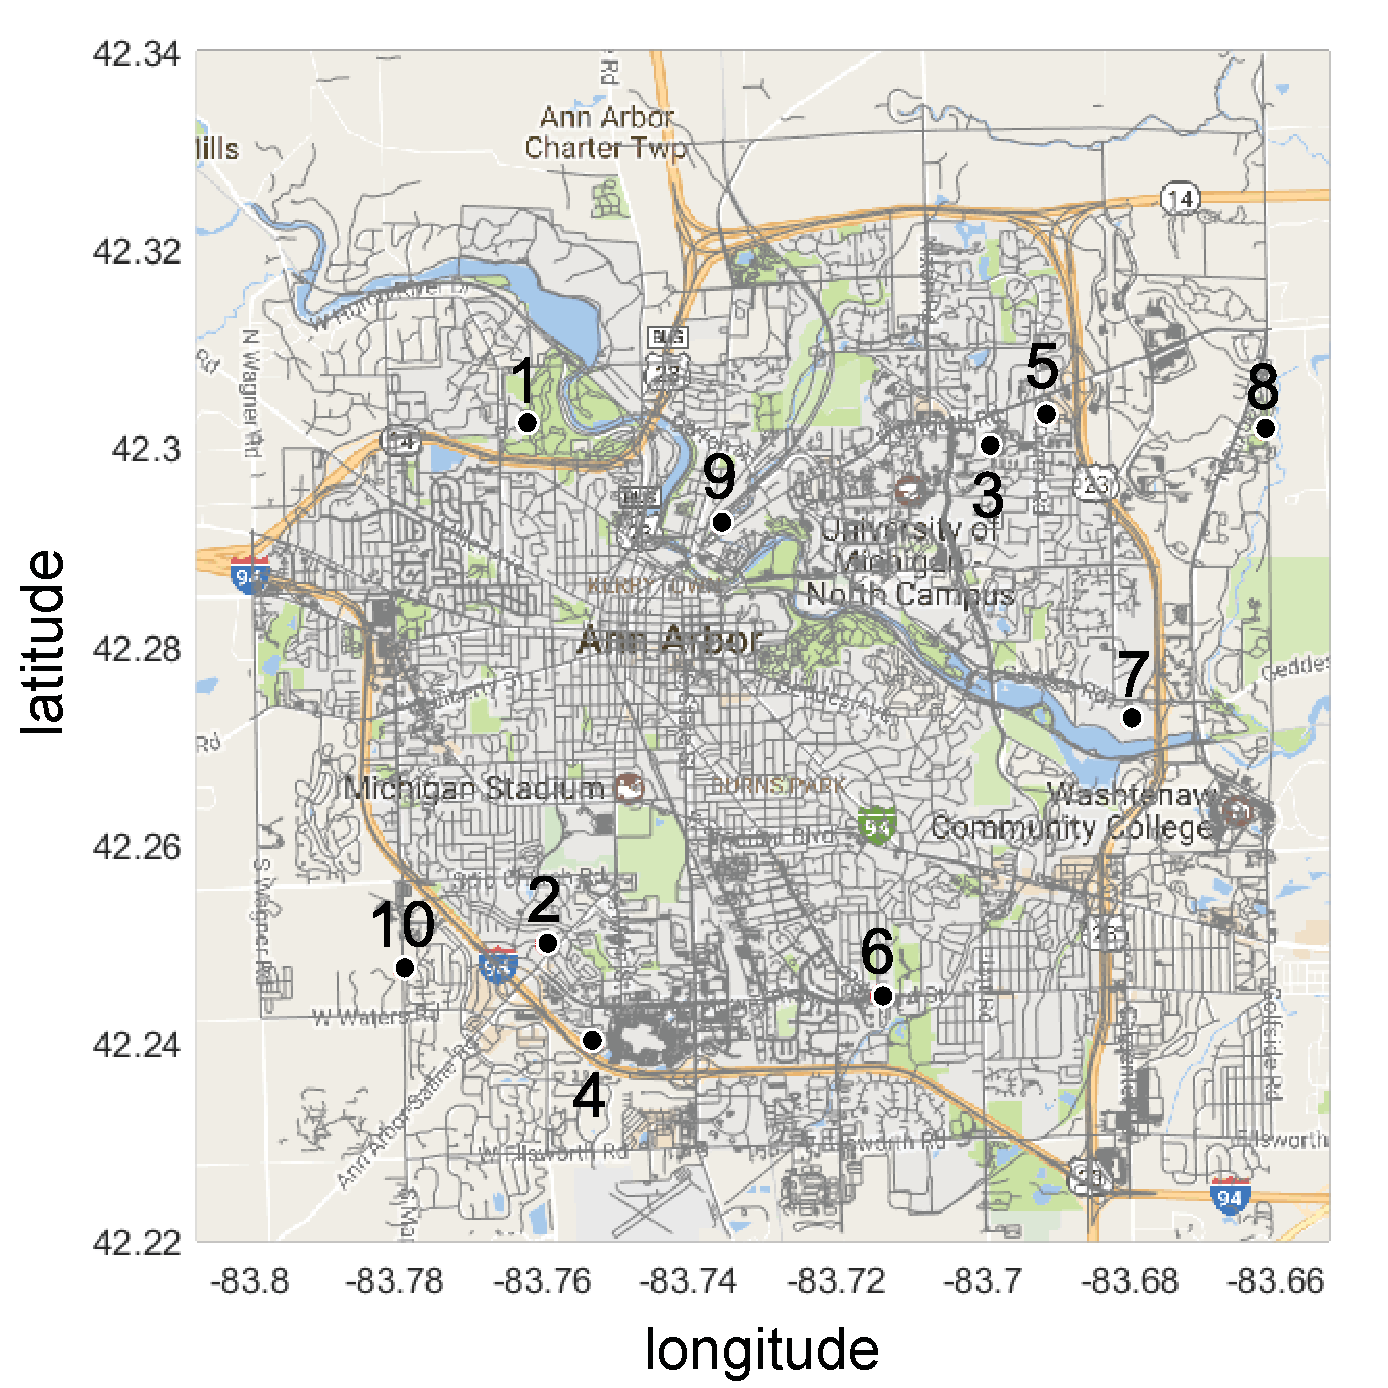
\includegraphics[width=2.6in]{figure/fig0}
\captionof{figure}{Initial configuration of 10 vehicles in Ann Arbor}
\label{fig:fig1}
\end{Figure}
If $\mathbf{x}^{\star}$ solves ($\star$) for along every time step, then 
using a similar argument as was used in \cite{bertsimas1993stochastic}, it is straightforward to show that for an arbitrary value of $k$, Algorithm \ref{thm:alg2} is \emph{asymptotically optimal} in the light load.
\section{Numerical Simulations}
For our simulations, we retrieved the road map of Ann Arbor from Open Street Maps (OSM)\cite{OpenStreetMap} database and represent the road map as an undirected graph, $\mathcal{G}(\mathcal{V},\,\mathcal{E})$. 
Fig. 1 shows 10 indexed vehicles, initially deployed in the city. For the $1^{\textup{st}}$ round of simulations, we assume that each demand arrives in $\mathcal{G}$ and the vehicles are \emph{not} confined to move in $\mathcal{G}$. Fig. 2 compares the configuration/induced partition of 10 vehicles after 40 iterations of gradient algorithm with $k=1$ {\color{black}{(\emph{state-of-the-art} method \cite{bertsimas1993stochastic})}} and $k=2$ (our \emph{robust} approach). {\color{black}{Fig. 3 compares the cost changes during iterations with $k=1$ and $k=2$, \emph{if the $1^{\textup{st}}$ vehicle is unavailable}, where we varied the value of $\overline{\sigma}$, namely, \emph{an expected service delay (an unmodeled cost) incurred due to the $1^{\textup{st}}$ vehicle's unavailability}. The figure illustrates that our method with $k=2$ is robust to service delay due to unavailability of a single vehicle.}}

Next, we consider the case when vehicles are confined to travel in $\mathcal{G}$. Two conspicuous problems arise if the constraint is enforced; 1) calculating the gradient becomes intractable (this is in large part due to the distance terms found in ($\star$)). We assume as an approximation that minimum distance between any two points on the $\mathcal{G}$ is {\color{black}{proportional}} to the Euclidean distance between them. 2) Since 
each vehicle must lie on $\mathcal{G}$ all the time, unless the algorithm converges to $m$-points on the road map, in general there is no feasible solution. Thus we consider nearest neighbor approximation, namely, to find $\hat{\mathbf{x}} = \arg\min_{\mathbf{x}\,:\,\mathbf{x}_i \in \overline{\mathcal{B}}(\mathbf{x}_i^{\star},\delta)\cap \mathcal{E}} H_k$ where $\delta > 0$. 
Fig. \ref{fig:fig4} (left) shows one-time deployment of 10 vehicles over $\mathcal{G}$ with $k=2$, and Fig. 4 (right) displays $9^{\textup{th}}$ vehicle's path in $\mathcal{G}$ in response to a demand generated at the square point, when $1^{\textup{st}}$ vehicle is unavailable. In this case, the $9^{\textup{th}}$ vehicle arrives to the demand instead in roughly $8$ minutes (GPS ranges shown in Fig. \ref{fig:fig4} for both coordinates are approximately 9.66 miles, and each vehicle travels at a constant speed $30$mph). The shortest paths were determined by Dijkstra's algorithm \cite{dijkstra1959note}.

\begin{Figure}
\centering
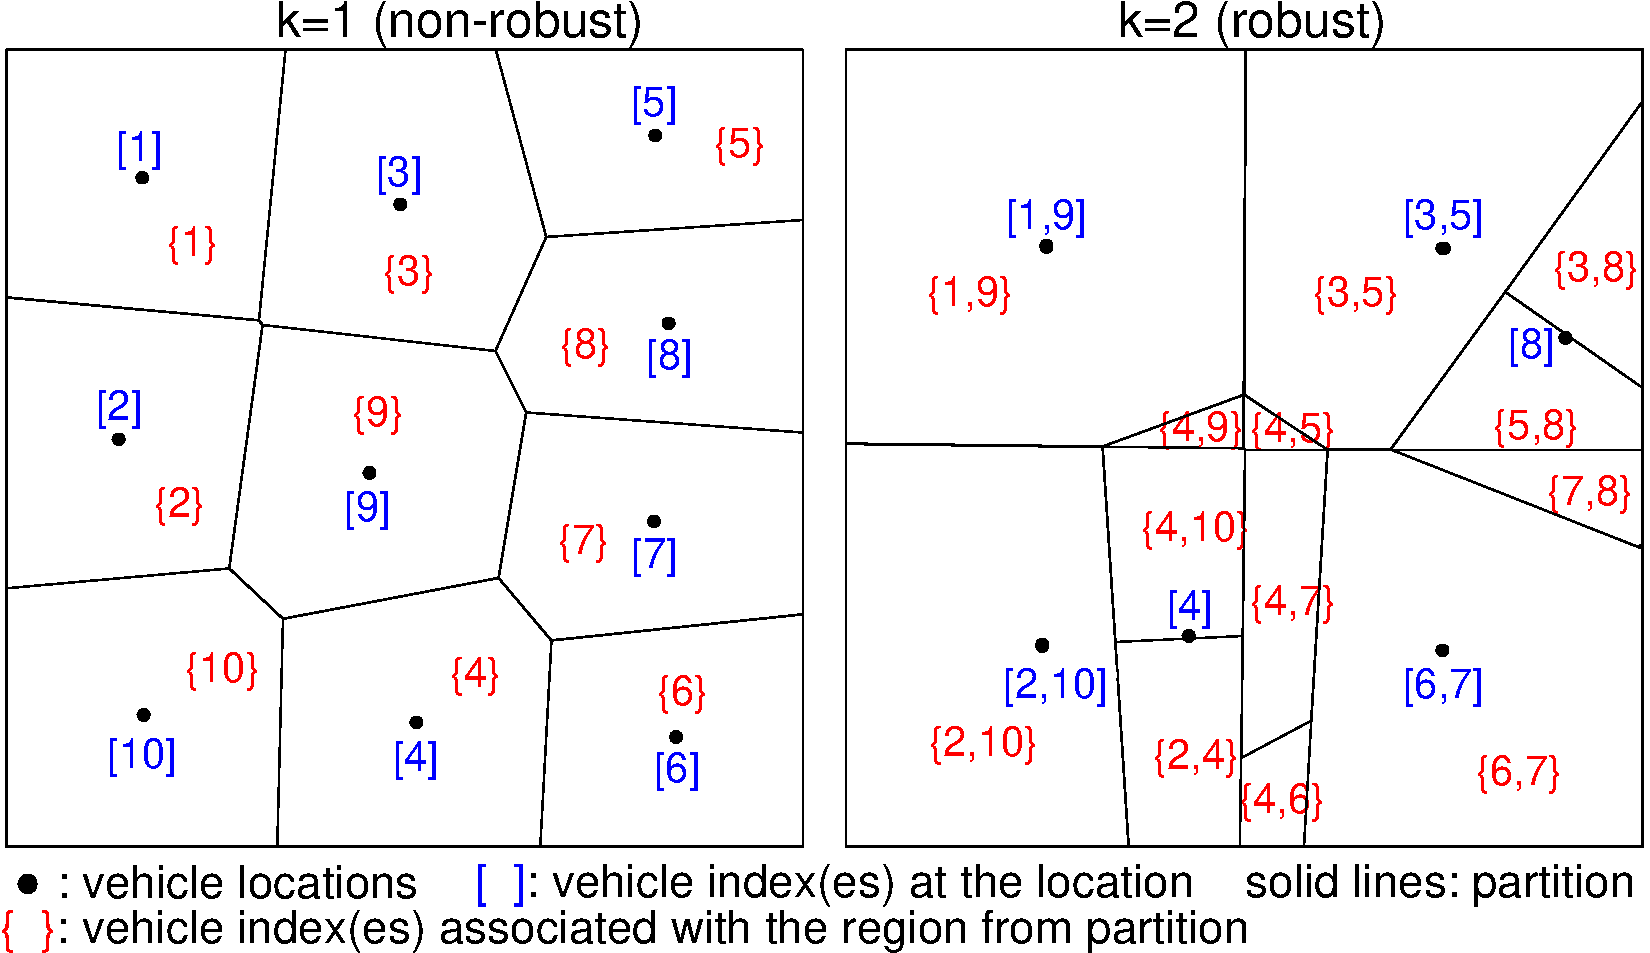
\includegraphics[width=4in]{figure/fig34}
\captionof{figure}{Vehicles' locations, induced partition after 40 iterations}
\label{fig:fig2}
\end{Figure}

\begin{Figure}
\centering
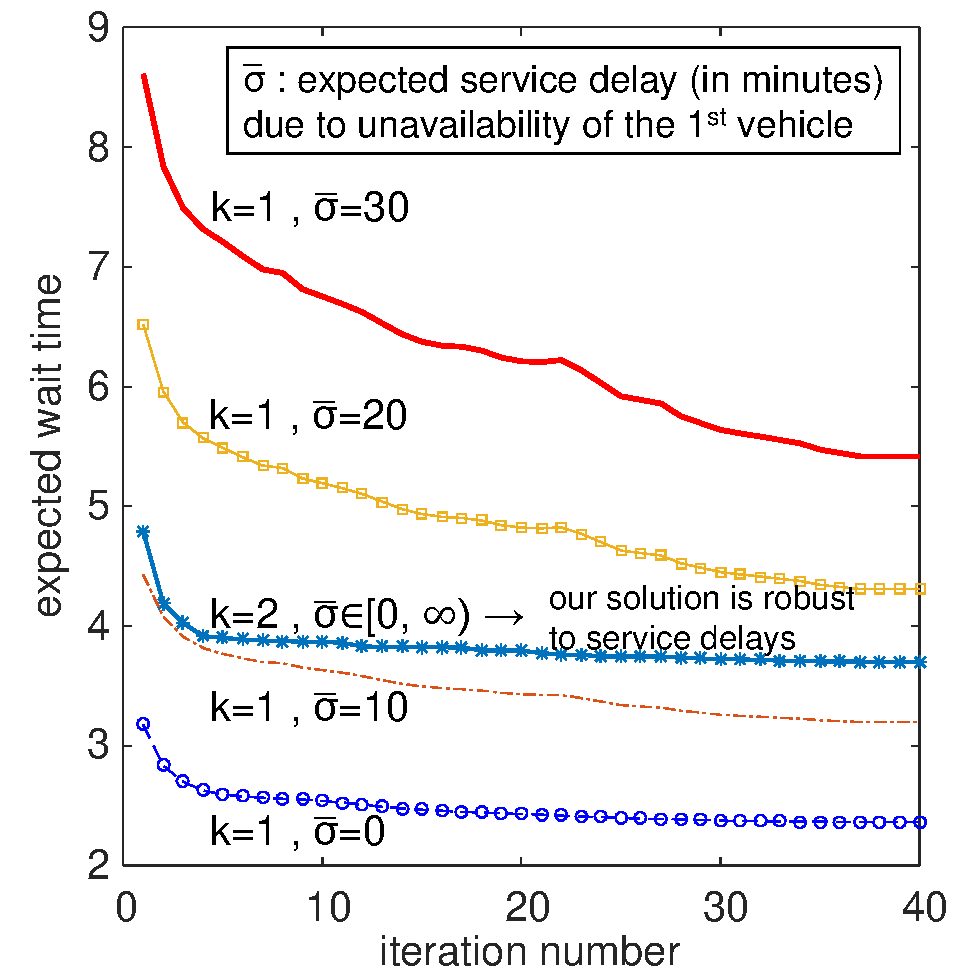
\includegraphics[width=2.6in]{figure/fig3l}
\captionof{figure}{Mean wait time with $k=1$, $k=2$ for different service delay values when the $1^{\textup{st}}$ vehicle is unavailable}
\label{fig:fig3}
\end{Figure}

\begin{Figure}
\centering
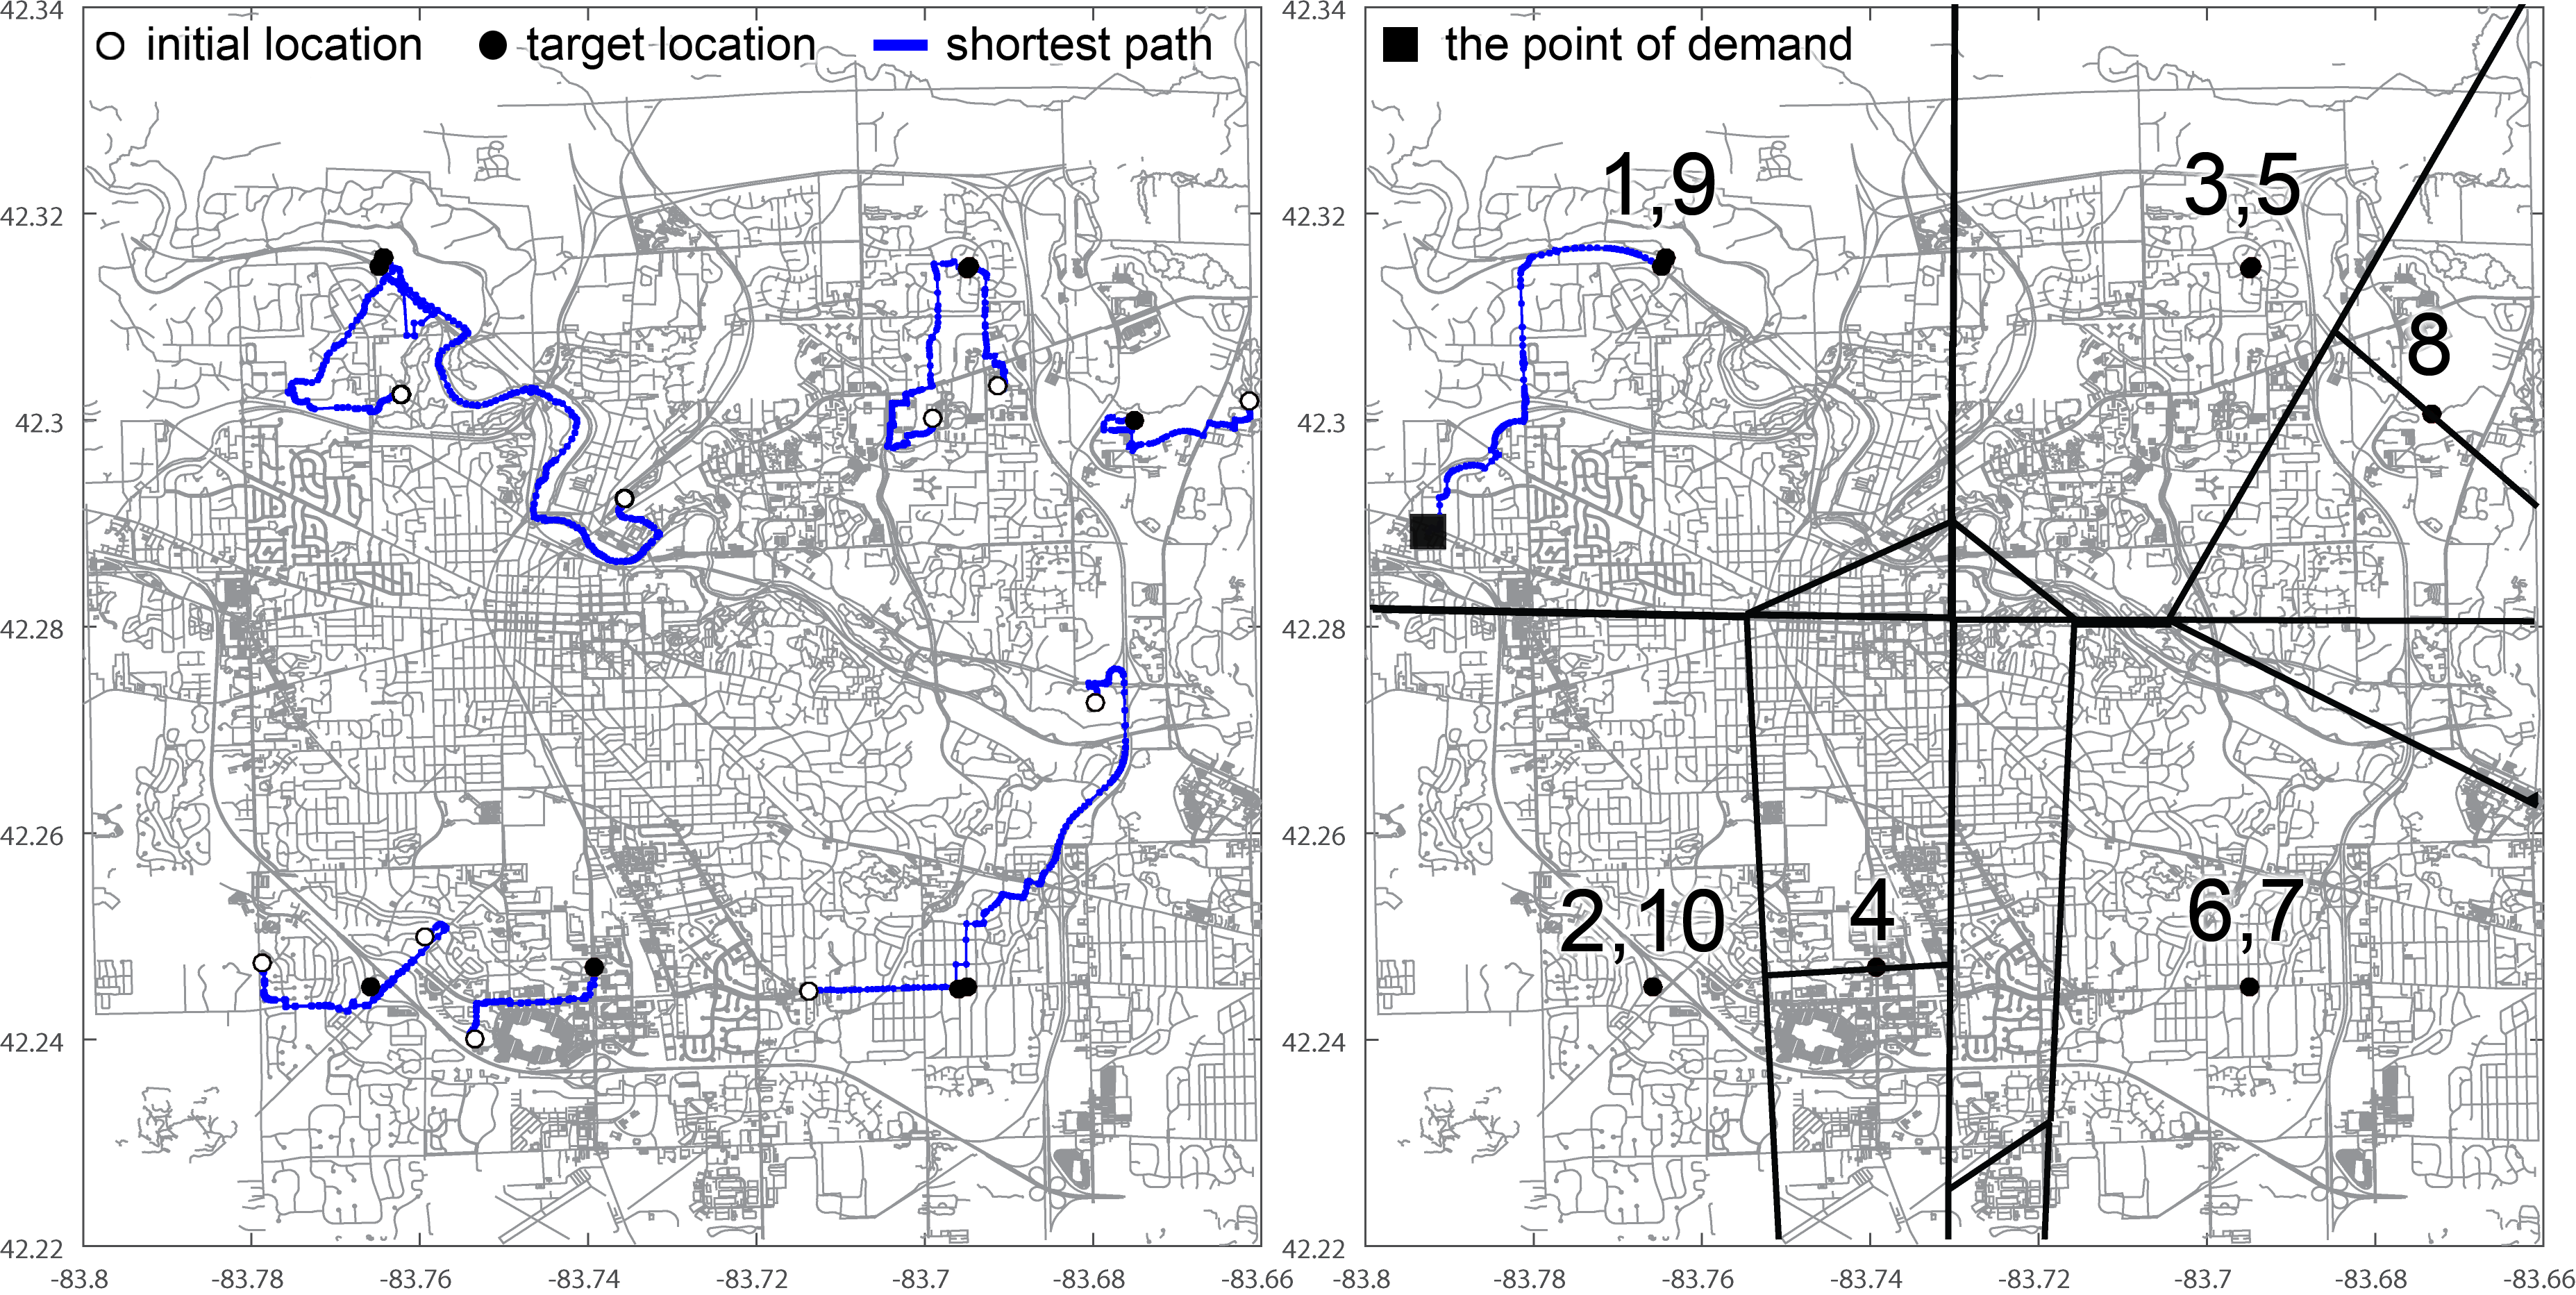
\includegraphics[width=5in]{figure/fig45_new3}
\captionof{figure}{left: one-time deployment over $\mathcal{G}$, right: response to a demand when $1^{\textup{st}}$ vehicle is unavailable where bold lines show the partition}
\label{fig:fig4}
\end{Figure}
\section{Discussion}
This paper presents a novel average-worst-case framework for the assignment of depots for DVR problem in light load.  Our method becomes unstable as the load increases, and obtaining the optimal solution requires  {\color{black}{a}} central entity. Future work will involve full consideration of various traffics conditions including congestion effects. 
In addition, it should be of independent interest to efficiently {\color{black}{adapt}} DVR policies to work under a road map constraint.

<<<<<<< HEAD
\section{Acknowledgments}
=======
\section{Acknowledgement}
>>>>>>> 92e34d0145ec7081c1a3d7ae929b431af16982d5
This work was supported by Ford Motor Company.

\bibliographystyle{IEEEtran}
\bibliography{ref}

\appendix
\section{Appendix: Proofs}
\begin{proof}[Proof of Theorem \ref{thm:thm1}]
Consider an arbitrary partition $\mathbb{W}=(W_1,\dots,W_l)$ of $\mathcal{Q}$ into $l$ regions where each region $W_i \subset \mathcal{Q}$ is assigned to $k$ generators, i.e., $k$ number of points from $\mathbf{x}$. Then, by the property of space partition, $W_i \cap W_j = \emptyset$ for every pair $i,\,j \in \lbrace 1,\dots,l \rbrace$ with $i \neq j$, and $\cup_i W_i = \mathcal{Q}$.
Consider a Voronoi partition of order $k$, namely $\mathbb{V}=(V_1,\dots,V_m)$, a partition of $\mathcal{Q}$ into $m$ regions, where each region is associated to $k$ points. 
We note here that given $\mathcal{Q}$ and a configuration $\mathbf{x} \in \mathcal{Q}^m$, the Voronoi diagram of order $k$ is an \emph{unique} tessellation of $\mathcal{Q}$ (for details see, e.g., \cite{okabe2009spatial}).
Recalling the definition of the order-$k$ Voronoi tessellation from \cite{okabe2009spatial}, it follows that 
\begin{equation}
V(\mathbf{z}) = \lbrace \mathbf{q} \,\mid\, \max_{\mathbf{p} \in \mathbf{z}} \left\| \mathbf{q}- \mathbf{p} \right\| \leq \min_{\mathbf{s} \in \mathbf{x} \setminus \mathbf{z}} \left\| \mathbf{q} - \mathbf{s} \right\| \rbrace,
\label{eq:vor}
\end{equation}
where $V(\mathbf{z})$ is read as a Voronoi polytope having $\mathbf{z}$ as its set of generators. 
To prove the theorem, we will show that for each point $\mathbf{q} \in \mathcal{Q}$, there is $\mathbf{z}$ satisfying (\ref{eq:vor}) such that the following inequality holds for all $\mathbf{y} \subset \mathbf{x}$ with $\left| \mathbf{y} \right| = k$
\begin{equation}
\max_{\mathbf{p} \in \mathbf{z}} \left\| \mathbf{q} - \mathbf{p} \right\| \leq 
\max_{\mathbf{r} \in \mathbf{y}} \left\| \mathbf{q} - \mathbf{r} \right\|,
\label{eq:showeq}
\end{equation}
where $\mathbf{y}$ is necessarily associated with a region from the arbitrary partition $\mathbb{W}$ of $\mathcal{Q}$, i.e., for the given partition $\mathbb{W}$ there exists $j \in \lbrace 1,\dots,l \rbrace$ such that $\mathbf{y}$ is associated with $W_j \in \mathbb{W}$.	
We address all three possible cases:
\begin{enumerate}[1)]
\item $\mathbf{y} = \mathbf{z}$: The equality from (\ref{eq:showeq}) holds trivially.
\item $\mathbf{y} \cap \mathbf{z} = \emptyset$: The inequality follows from (\ref{eq:showeq}) trivially from (\ref{eq:vor}).
\item $\mathbf{y} \cap \mathbf{z} \neq \emptyset$: This case needs further analysis. 
The equation (\ref{eq:vor}) implies that for all point $\mathbf{s} \in \mathbf{x} \setminus \mathbf{z}$,
\begin{align*}
\max_{\mathbf{p} \in \mathbf{z} } \left\| \mathbf{q}-\mathbf{p} \right\| \leq \left\| \mathbf{q} - \mathbf{s} \right\|,
\end{align*}
such that
\begin{equation}
\max_{\mathbf{p} \in \mathbf{z} } \left\| \mathbf{q}- \mathbf{p} \right\| \leq
\min_{\mathbf{v} \in \mathbf{y} \setminus \mathbf{z}}\left\| \mathbf{q} - \mathbf{v} \right\|.
\label{eq:eq1}
\end{equation}
Using the property of max operator, we have
\begin{equation}
\max_{\mathbf{w} \in \mathbf{z}\cap \mathbf{y}} \left\| \mathbf{q} - \mathbf{w} \right\| \leq \max_{\mathbf{p} \in \mathbf{z}} \left\| \mathbf{q} - \mathbf{p} \right\|.
\label{eq:eq2}
\end{equation}
Combining (\ref{eq:eq1}) and (\ref{eq:eq2}), gives
\[
\max_{\mathbf{p} \in \mathbf{z} } \left\| \mathbf{q}- \mathbf{p}\right\| 
\leq 
\max \left\{ \min_{\mathbf{v} \in \mathbf{y} \setminus \mathbf{z}}\left\| \mathbf{q} - \mathbf{v} \right\| ,\,\max_{\mathbf{w} \in \mathbf{z}\cap \mathbf{y}} \left\| \mathbf{q} - \mathbf{w} \right\| \right\}\leq \max_{\mathbf{r} \in \mathbf{y}} \left\| \mathbf{q}- \mathbf{r} \right\|.
\]
Thus,
\begin{equation}
\mathbf{z} = \arg \min_{\mathbf{y} \subset \mathbf{x},\left| \mathbf{y} \right| =k}\max_{\mathbf{r} \in \mathbf{y}} \left\| \mathbf{q}- \mathbf{r} \right\|.
\label{eq:fin}
\end{equation}
\end{enumerate}	
Hence, given an arbitrary partition $\mathbb{W}= (W_1,\dots,W_l)$ of $\mathcal{Q}$, for each $\mathbf{q} \in W_j$ where $j \in \lbrace 1,\dots,l \rbrace$, there is a unique set of $k$ points $\mathbf{z} \subset \mathbf{x}$ and its associated order-$k$ Voronoi region $V(\mathbf{z}) \in \mathbb{V}$ such that (\ref{eq:fin}) holds. Since this property holds for any configuration $\mathbf{x} \in \mathcal{Q}^m$, $\mathbb{V}$ is the optimal partition for ($\star$). 
\end{proof}

\begin{lemma}
For each $i \in I$, $k \in I$,
\begin{align}
&\frac{\partial
	H_k([\cdots,\mathbf{x}_i,\cdots]^{\top},\,\mathcal{Q})
}{\partial
	\mathbf{x}_i
} =-\int_{G_k(\lbrace \mathbf{x}_i \rbrace )\setminus G_{k-1}( \lbrace \mathbf{x}_i \rbrace )}\frac{1}{\left\| \mathbf{q} - \mathbf{x}_i \right\|}
(\mathbf{q} - \mathbf{x}_i )\phi(\mathbf{q})\,\mathbf{dq}.
\label{eq:eq13}
\end{align}
\label{thm:lem1}
\end{lemma}
The proof of Lemma \ref{thm:lem1} depends on the following two propositions.
\begin{proposition}
For each $k \in I$
\begin{equation}
\lbrace G_k(\lbrace \mathbf{x}_i \rbrace ) \setminus G_{k-1}(\lbrace \mathbf{x}_i \rbrace) \rbrace_{i=1}^m
\label{eq:eq08}
\end{equation}
is a partition of $\mathcal{Q}$.
\label{thm:prop1}
\end{proposition}
\begin{proof}[Proof of Proposition \ref{thm:prop1}]
We note without proof \cite{okabe2009spatial} that $\mathbb{W} = (W_1,\dots,W_l)$ is a partition of $\mathcal{Q} \subseteq \Re^d$ if and only if, $W_j \subseteq \mathcal{Q}$ for all $j \in \lbrace 1,\dots,l \rbrace$, and 
\begin{equation}
\sum_{i=1}^l \int_{W_i} \mathbf{dq} = \int_{\mathcal{Q}} \mathbf{dq}.
\label{eq:eq09}
\end{equation}
Also, it is routine to verify---using the definition of the order-$k$ Voronoi tessellation (\ref{eq:vor})---that for every $k \in I$,
\begin{equation}
\sum_{i=1}^m \int_{G_k(\lbrace \mathbf{x}_i \rbrace )} \mathbf{dq} = k \times \int_{\mathcal{Q}} \mathbf{dq}.
\label{eq:eq10}
\end{equation}
First, we show that for each $k \in I$, and $i \in I$,
\begin{equation}
G_{k-1}(\lbrace \mathbf{x}_i \rbrace) \subseteq G_k(\lbrace \mathbf{x}_i \rbrace ) 
\label{eq:eq11}
\end{equation}
If $\mathbf{q} \in G_{k-1}(\lbrace \mathbf{x}_i \rbrace)$, then again by the definition of the order-$k$ Voronoi tessellation (\ref{eq:vor}),
\[
\left\| \mathbf{q} - \mathbf{x}_i \right\|
\leq 
\max_{\mathbf{x}_j \in G_{k-1}^{-1}(\lbrace \mathbf{q} \rbrace)}\left\| \mathbf{q} - \mathbf{x}_j \right\| \leq \min_{\mathbf{x}_l \in \mathbf{x} \setminus G_{k-1}^{-1}(\lbrace \mathbf{q} \rbrace)} \left\| \mathbf{q} - \mathbf{x}_l \right\|.
\]
By using the properties of min, max operators, we have
\[
\left\| \mathbf{q} - \mathbf{x}_i \right\|
\leq 
\max_{\mathbf{x}_j \in G_{k-1}^{-1}(\lbrace \mathbf{q} \rbrace)}\left\| \mathbf{q} - \mathbf{x}_j \right\| \leq 
\max_{\mathbf{x}_j \in G_{k}^{-1}(\lbrace \mathbf{q} \rbrace)}\left\| \mathbf{q} - \mathbf{x}_j \right\| \leq 
\min_{\mathbf{x}_l \in \mathbf{x} \setminus G_{k}^{-1}(\lbrace \mathbf{q} \rbrace)} \left\| \mathbf{q} - \mathbf{x}_l \right\| \leq
\min_{\mathbf{x}_l \in \mathbf{x} \setminus G_{k-1}^{-1}(\lbrace \mathbf{q} \rbrace)} \left\| \mathbf{q} - \mathbf{x}_l \right\|.
\]
Hence, $
\mathbf{q} \in G_{k}(\mathbf{x}_i)
$, and this implies (\ref{eq:eq11}).
By using the spatial relationships (\ref{eq:eq10}) and (\ref{eq:eq11}), we have
\begin{align*}
\sum_{i=1}^m \int_{G_k(\lbrace \mathbf{x}_i \rbrace )} \mathbf{dq} & =\sum_{i=1}^m \int_{G_k( \rbrace \mathbf{x}_i \rbrace )\setminus G_{k-1}(\lbrace \mathbf{x}_i \rbrace )} \mathbf{dq} + \underbrace{\int_{G_{k-1}(\lbrace \mathbf{x}_i\rbrace )}}_{(k-1) \times \int_{\mathcal{Q}} \mathbf{dq}} \mathbf{dq} = k\times \int_{\mathcal{Q}} \mathbf{dq}.
\end{align*}
Hence,
$
\sum_{i=1}^m \int_{G_k(\lbrace \mathbf{x}_i \rbrace )\setminus G_{k-1}(\lbrace \mathbf{x}_i \rbrace )} \mathbf{dq} = \int_{\mathcal{Q}} \mathbf{dq}.
$
By using the property of the space partitioning (\ref{eq:eq09}), we can conclude that (\ref{eq:eq08}) is a \emph{partition} of $\mathcal{Q}$.
\end{proof}
\begin{proposition}
Let
\begin{equation}
\mathcal{U} = \lbrace \mathbf{q} \in \mathcal{Q}\,\mid\,\mathbf{q} \in G_{k}(\mathbf{x}_i) \setminus G_{k-1}(\lbrace \mathbf{x}_i \rbrace) \rbrace.
\label{eq:eq0}
\end{equation}
Then, for each $\mathbf{q} \in \mathcal{U}$, $	\mathbf{x}_i = \arg\max_{\mathbf{x}_j \in G_{k}^{-1}(\mathcal{U}) } \left\| \mathbf{q}- \mathbf{x}_j \right\|.$
\label{thm:prop2}
\end{proposition}
\begin{proof}[Proof of Proposition \ref{thm:prop2}]
Suppose towards contradiction that there exists $\mathbf{x}_l \neq \mathbf{x}_i$ and $\mathbf{q} \in \mathcal{U}$ such that 
\begin{equation}
\mathbf{x}_j = \arg\max_{\mathbf{x}_j \in G_{k}^{-1}(\mathcal{U}) } \left\| \mathbf{q}- \mathbf{x}_j \right\|.
\label{eq:eq07}
\end{equation}
Then, according to the definition of the order-$k$ Voronoi tessellation (\ref{eq:vor}), (\ref{eq:eq07}) implies that $\mathbf{x}_l$ is exactly the $k$th nearest generator in distance to $\mathbf{q}$; however, it is immediate from the definition of the set $\mathcal{U}$ from (\ref{eq:eq0}) that $\mathbf{x}_i$ is the $k$ nearest generator to $\mathbf{q}$. Hence $\mathbf{x}_l = \mathbf{x}_i$, and a contradiction is obtained.
\end{proof}
Now we are ready to prove Lemma \ref{thm:lem1}.

\begin{proof}[Proof of Lemma \ref{thm:lem1}]
Recall that 
\begin{align}
&\mathbb{E}
\left[
\min_{i \in I }
\underset{i \in S:\atop \, S \subset I,\,\left|S\right|=k}{\max}
\left\| \mathbf{q}- \mathbf{x}_i \right\|
\right]=
\sum_{V\in \mathbb{V}}\int_{V} 
\underset{i \in I:\atop \mathbf{x}_i \in G_k^{-1}(V)}{\max}
\left\| \mathbf{q} - \mathbf{x}_i \right\| \phi(\mathbf{q})\,\mathbf{dq}.
\label{eq:eqeq1}
\end{align}
Using Proposition \ref{thm:prop1} and \ref{thm:prop2}, we can simplify the right-hand side of (\ref{eq:eqeq1}) as follows:
\begin{align*}
H_k(\mathbf{x},\,\mathcal{Q})
&= \sum_{V\in \mathbb{V}}\int_{V} 
\underset{i \in I:\atop \mathbf{x}_i \in G_k^{-1}(V)}{\max}
\left\| \mathbf{q} - \mathbf{x}_i \right\| \phi(\mathbf{q})\,\mathbf{dq} & \textup{[by Proposition \ref{thm:prop1}]} \\
&= \sum_{i=1}^m \int_{G_k(\lbrace \mathbf{x}_i \rbrace ) \setminus G_{k-1}(\lbrace \mathbf{x}_i \rbrace )}
\left(\max_{\mathbf{x}_j \in G_{k}^{-1}(
	G_k(\lbrace \mathbf{x}_i \rbrace ) \setminus G_{k-1}(\lbrace \mathbf{x}_i \rbrace)) } \left\| \mathbf{q}- \mathbf{x}_j \right\| \right) \phi(\mathbf{q})\,\mathbf{dq} \, & \textup{[by Proposition \ref{thm:prop2}]} \\
&= \sum_{i=1}^m \int_{G_k(\lbrace \mathbf{x}_i \rbrace ) \setminus G_{k-1}(\lbrace \mathbf{x}_i \rbrace )} 
\left\|\mathbf{q}- \mathbf{x}_i \right\| \phi(\mathbf{q})\,\mathbf{dq}.
\end{align*}
After a simple differentiation with respect to each coordinate vector $\mathbf{x}_i$, we have for each $k \in I$, $i \in I$:
\begin{align*}
\frac{\partial
	H_k([\cdots,\mathbf{x}_i,\cdots]^{\top},\,\mathcal{Q})
}{\partial
	\mathbf{x}_i
} = -\int_{G_k(\lbrace \mathbf{x}_i \rbrace)\setminus G_{k-1}(\lbrace \mathbf{x}_i \rbrace)}\frac{1}{\left\| \mathbf{q} - \mathbf{x}_i \right\|}
(\mathbf{q} - \mathbf{x}_i )\phi(\mathbf{q})\,\mathbf{dq}.
\end{align*}
\end{proof}

\end{document}
